\section{評価結果}
今回倉庫棚を想定した棚での飛行実験は安定して想定通りの経路を飛行を行う事が出来た\footnote{\url{https://youtu.be/pw23Vq8DuHE}}.
具飛行成績表を以下に示す.\ref{table:fly_result}

\begin{table}[h]
    \caption{飛行結果}
    \label{table:fly_result}
    \centering
    \begin{tabular}{cccc}
        \hline
        試行回数 & 到達可否 & 周回時間[sec] & 平均位置補正時間[sec] \\
        \hline \hline
        1回目 & 可 & 214.58 & 12.22 \\
        2回目 & 可 & 199.19 & 10.08 \\
        3回目 & 可 & 225.43 & 12.35 \\
        4回目 & 可 & 242.86 & 14.20 \\
        5回目 & 可 & 289.67 & 19.44 \\
        6回目 & 可 & 294.40 & 19.97 \\
        7回目 & 可 & 285.03 & 18.93 \\
        8回目 & 可 & 265.28 & 16.76 \\
        9回目 & 可 & 269.05 & 17.20 \\
        10回目 & 可 & 313.89 & 22.10 \\
        \hline
    \end{tabular}
\end{table}

コースを10周した時の1周あたりの時間のグラフを以下に示す.\ref{rap_plot}

\begin{figure}[htbp]
  \begin{center}
    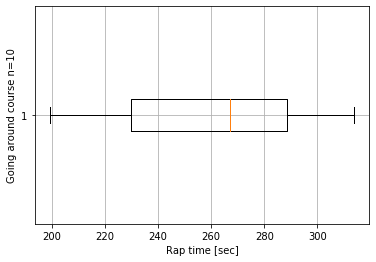
\includegraphics[clip,width=15.0cm]{img/rapdata.png}
    \caption{コースの周回時間}
    \label{rap_plot}
  \end{center}
\end{figure}

位置補正の時間計測に関して初回の位置合わせに時間がかかる事が多いものの,二つ目以降の位置合わせには時間差はあまり出なかった.
以下に90回分の位置補正にかかった時間データの箱ひげ図を示す.\ref{postime_plot}

\begin{figure}[htbp]
    \begin{center}
      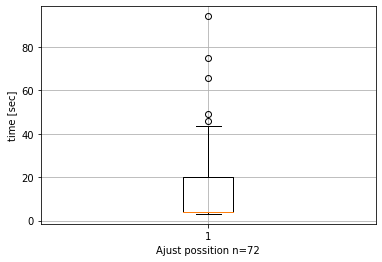
\includegraphics[clip,width=15.0cm]{img/timedata.png}
      \caption{位置補正に要した時間}
      \label{postime_plot}
    \end{center}
  \end{figure}

  多くの場合において20秒以内に位置補正が完了している事が分かる.